\chapter{Análisis de las correlaciones entre las distintas métricas}\label{chapter:correlations}
\addcontentsline{toc}{chapter}{Análisis de las correlaciones entre las distintas métricas}

En primer, las correlaciones que más nos interesan son las de las distintas métricas con la variable \emph{Grade}. En la Figura \ref{fig:correlations} podemos ver que no todas las métricas clásicas correlan con la misma. Nótese que es difícil encontrar métricas que correlen con la variable \emph{Grade} al ser ésta una medida subjetiva que contempla no sólo el rendimiento del alumnado en el servidor sino otros aspectos como la memoria de las prácticas, la presentación realizada de la misma, etc.

\begin{figure}[H]
    \centering
    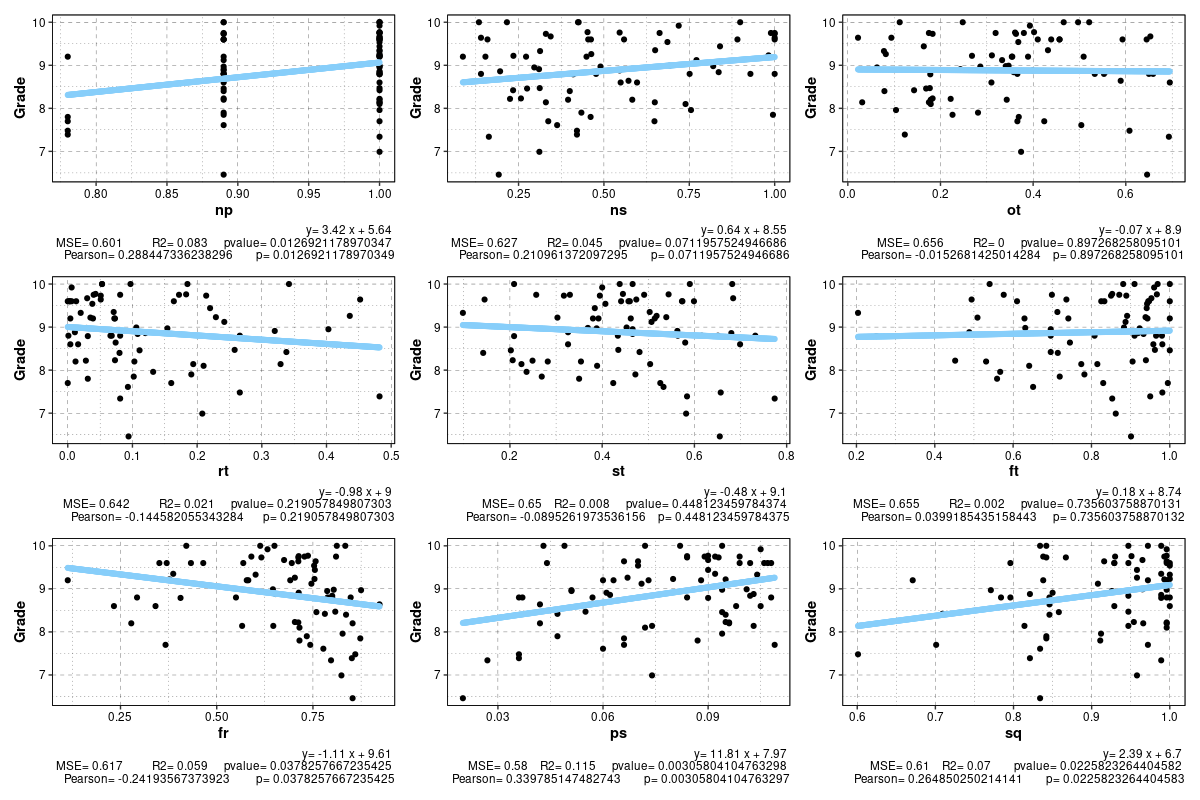
\includegraphics[width=\textwidth]{correlaciones/classicallinear.png}
    \caption{Correlaciones existentes entre las distintas métricas clásicas y la variable \emph{Grade}.}
    \label{fig:correlations}
\end{figure}

Así pues, vemos que las variables \emph{np} ($p = 0.0127 < 0.05$), \emph{fr} ($p = 0.0378 < 0.05$), \emph{ps} ($p = 0.0031 < 0.05$) y \emph{sq} ($p = 0.0226 < 0.05$) correlan con la calificación obtenida y que la variable \emph{ns} podría correlar con la variable \emph{Grade} aunque con un grado de certeza menor que el resto ($p = 0.0712 < 0.1$).

Además, realizando una regresión polinomial de orden $2$ entre dichas medidas y la variable \emph{Grade} obtenemos que existe una relación no lineal entre las variables \emph{np} ($p = 0.0137 < 0.05$), \emph{fr} ($p = 0.0016 < 0.05$) y \emph{ps} ($p = 0.0006 < 0.05$) y las calificaciones obtenidas tal y como se muestra en la Figura \ref{fig:correlations2}. Adicionalmente, podría existir una relación no lineal entre la variable \emph{sq} y la variable \emph{Grade} aunque con un grado de certeza menor ($p = 0.0695 < 0.1$).

\begin{figure}[H]
    \centering
    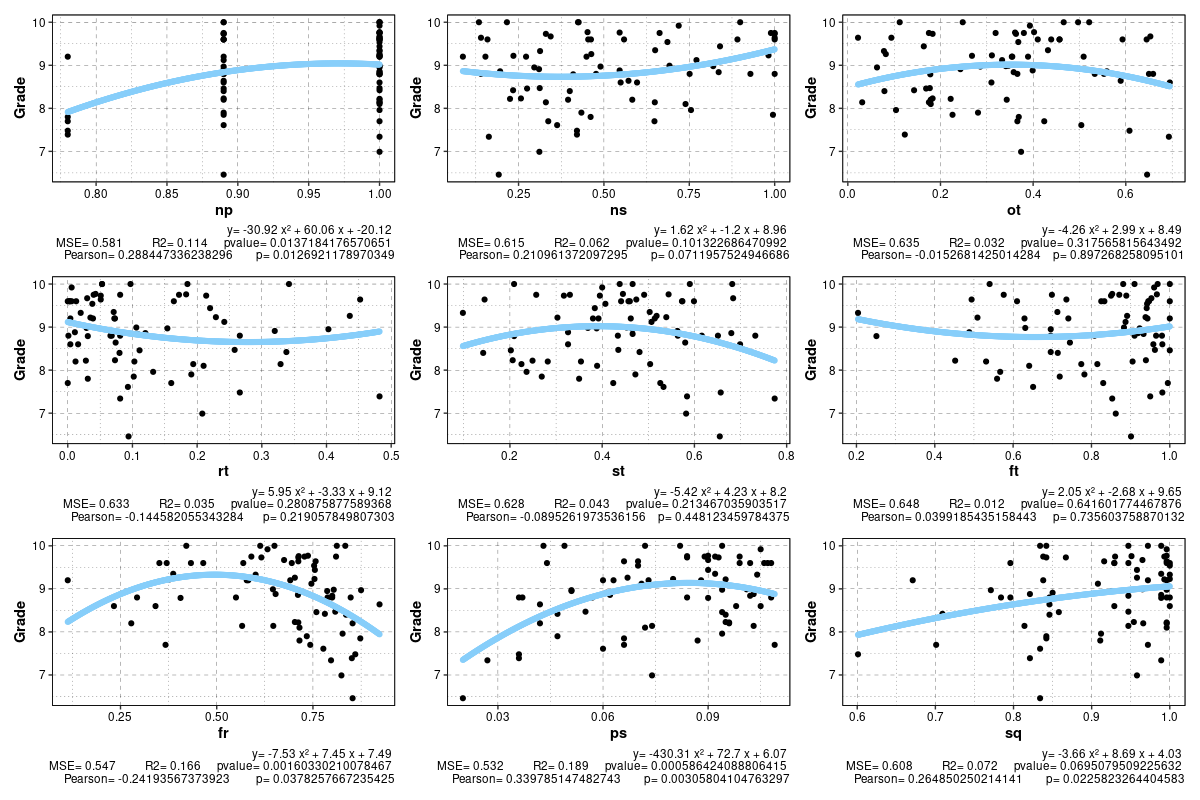
\includegraphics[width=\textwidth]{correlaciones/classicalpolynomial.png}
    \caption{Regresión polinomial de orden $2$ entre las distintas métricas clásicas y la variable \emph{Grade}.}
    \label{fig:correlations2}
\end{figure}

También estudiaremos las correlaciones existentes entre las medidas basadas en el análisis espectral de grafos y la variable \emph{Grade}. Empezaremos estudiando la correlación lineal entre las medidas anteriormente presentadas en la Sección \ref{sec:complexity} y la calificación obtenida por los distintos grupos de prácticas. Como vemos en la Figura \ref{fig:correlations3}, únicamente existe una relación lineal positiva entre las variables \emph{We} y \emph{Grade} ($p = 0.0374 < 0.05$).

\begin{figure}[H]
    \centering
    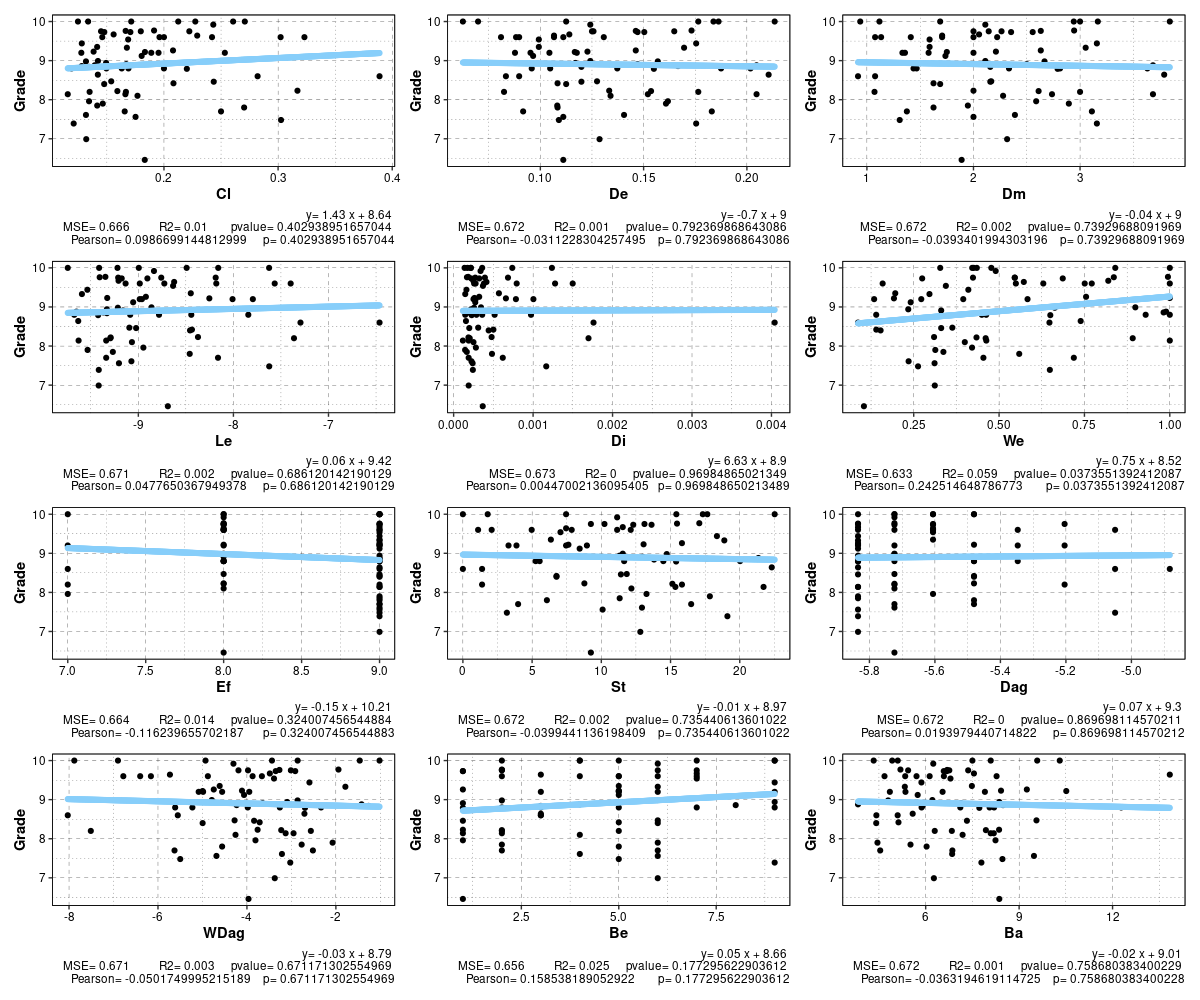
\includegraphics[width=\textwidth]{correlaciones/topologicallinear.png}
    \caption{Correlaciones existentes entre las medidas de complejidad de propósito general y la variable \emph{Grade}.}
    \label{fig:correlations3}
\end{figure}

Por último, estudiaremos si existe alguna relación no lineal entre alguna de las medidas topológicas estudiadas y las calificaciones obtenidas por el alumnado. Así pues, en la Figura \ref{fig:correlations4} podemos concluir que podría existir una relación no lineal entre las variables \emph{We} y \emph{Grade} ($p = 0.0774 < 0.1$).

\begin{figure}[H]
    \centering
    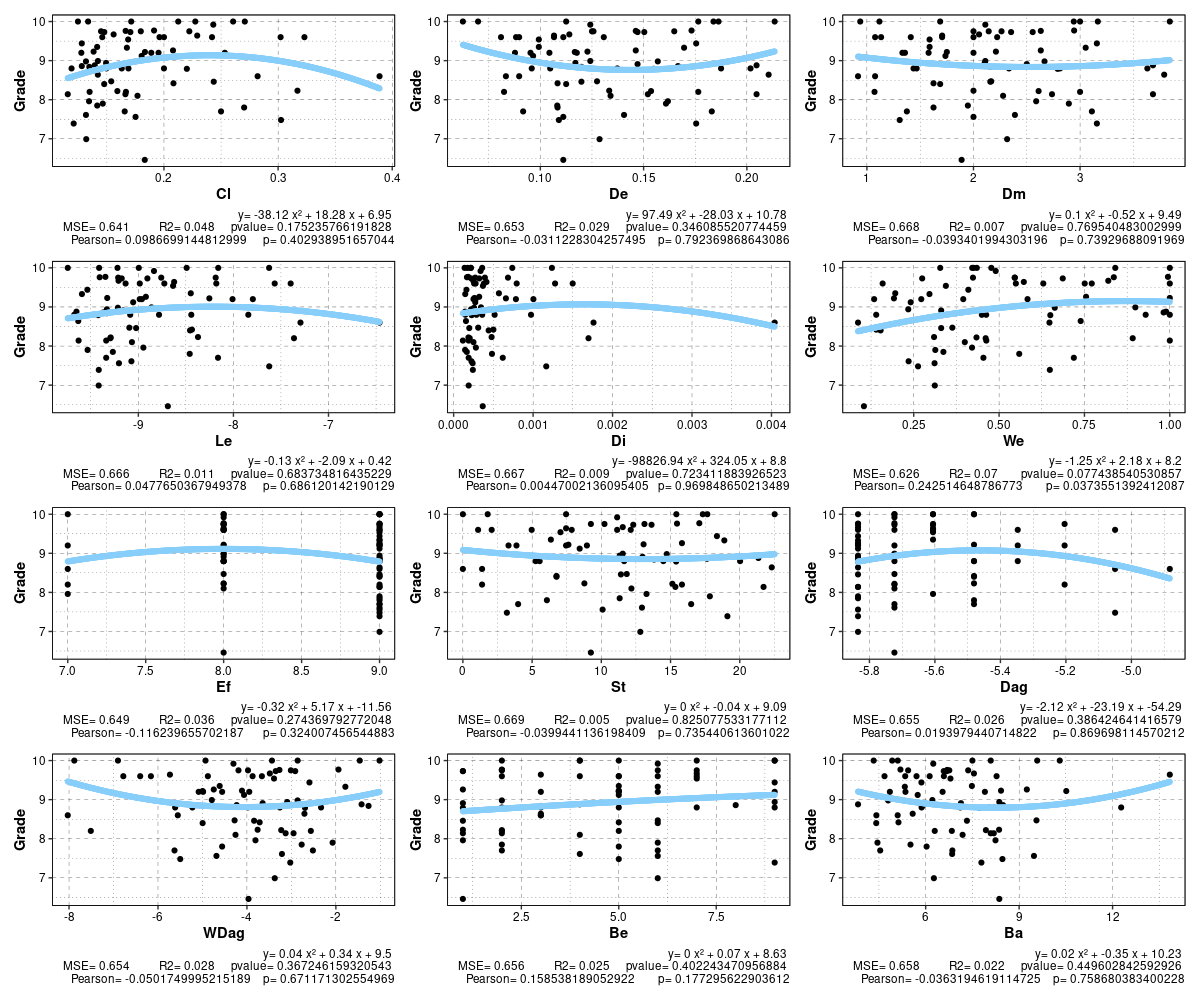
\includegraphics[width=\textwidth]{correlaciones/topologicalpolynomial.png}
    \caption{Regresión polinomial de orden $2$ entre las medidas de complejidad de propósito general y la variable \emph{Grade}.}
    \label{fig:correlations4}
\end{figure}